\subsection{Dispersion}

The most commonly available observable for the operator to set-up a beam line is the
centroid beam position and the beam intensity along the beam line, 
i.e. the beam orbit and transmission. 
At CTF3 this is mainly measured by Beam Position Monitors (BPMs) installed
in the different lines.
At start-up, the hope of the operator is that the transverse optics and the beam quality
are good enough to be able to transport the beam all the way without major beam losses.
This is normally achieved after a few empirical iterations acting on orbit corrector
magnets to steer the beam close to the centre of BPMs and, if necessary, slightly
adjusting the quadrupoles' strength.

Once the beam is transported all the way on a ``reasonable'' orbit, a useful verification
of the quality of the set-up can be achieved by means of dispersion measurements, i.e. the
orbit deviation of a particle due to its energy deviation with respect to the design
energy.
This is specially important in lines where dispersion is non-zero by design, 
like in the Drive Beam Recombination Complex (DBRC). 
An uncontrolled dispersion may easily increase the transverse beam size, 
leading to heavy beam losses and degraded stability.
At CTF3 a MATLAB application has been developed to perform \emph{online} dispersion
measurements in the different beam lines.
The final functionalities and design of this application is the result of various
iterations to respond to the needs raised during daily CTF3 operations.
Before describing the main features and use of the application
the basic concepts and techniques used for these measurements are discussed.


%%%%%%%%%%%%%%%%%%%%%%%%%%%%%%%%%%%%%%%%%%%%%%%%%%%%%%
\subsubsection{Common notions for dispersion measurement}
\label{sub:detailDispMeas}
%
Some theoretical details about transverse phase-space energy dependence have been treated
in~\cite{bib:DavideThesis}, to which we will refer in the following paragraph.
By definition~\cite{Minty_Zimmermann_Book} the dispersion is the variation of the orbit of a single
off-energy particle, with respect to the orbit of a particle with nominal energy.
In the most general case the dispersion is a non-linear multi-dimensional function of the
phase-space coordinates in terms of the momentum offset ($x = D(\Delta p/p_0)$).
In the simpler linear case it is the linear coefficient $D_x$ in the relation:
\begin{align}
\Delta x_i = D_x \frac{\Delta p_i}{p_0}
\label{eq:simpleLinearDispersionDefinition}
\end{align}
where $\Delta x_i$ is the orbit displacement of the $i$\textsuperscript{th} particle due
to its energy offset $\Delta p_i/p_0$.
In first approximation one can see the full beam as a single particle with energy equal to
its mean energy.  
In order to measure the dispersion in a transfer line, experimentally one has to change
the energy of the beam with respect to the nominal energy for which the line is tuned,
and so measure the effect on the mean beam orbit.
At CTF3 this can be accomplished in different ways:
%
\begin{itemize}
\item
By scaling all the magnetic elements of the transfer line under consideration. This does
not change the properties of the beam, but the scaled strength of the magnetic elements
will give the same effect as an inverse change in the energy of the beam. 
Note that this method will not reveal a possible incoming dispersion if the scaling is
performed only on a section of the line.
Moreover, as shown in~\cite{bib:DavideThesis}, this method is valid only for measuring
the first-order dispersion.
\item
By scaling the beam current at the source. Since the Drive Beam linac relies on fully
loaded acceleration, any change in beam current is translated in an effective mean energy
variation\footnote{By scaling the beam current one might also induce some other
intensity-related orbits effect, like wake fields kicks. This has been used for Wakefield
Free Steering (WFS) in \cite{Latina:2014jca, Latina:2014ama}.} that can be assumed to be
linear \cite{bib:CTF3DesignReport}.
\item
By moving the RF phase and/or power of one accelerating structure. This will simply lead
to a smaller acceleration at one location of the linac, and so a final variation of beam
energy. This measurement would start only from the chosen structure onward, and normally
one could obtain slightly different results depending on the chosen structure.
\item
Parasitically, by watching the natural shot-to-shot beam-energy jitter due to RF phase, 
RF power jitter and/or beam current jitter.
\end{itemize}
%
From a mathematical point of view all these methods are similar and can be described by a
simple matrix formalism:
%
\begin{align}
\vec{a} &= (a_1; a_2; a_3; \ldots; a_n) \\
%
\mathbf{M} &=
\begin{bmatrix}
   b_{1,1} & b_{1,2} & b_{1,3} & \ldots & b_{1,n} \\
   b_{2,1} & b_{2,2} & b_{2,3} & \ldots & b_{2,n} \\
   b_{3,1} & b_{3,2} & b_{3,3} & \ldots & b_{3,n} \\
   \vdots &\vdots &\vdots &\cdots &\vdots \\
   b_{m,1} & b_{m,2} & b_{m,3} & \ldots & b_{m,n} \\
\end{bmatrix}
\end{align}
%
where $\mathbf{M}$ contains the beam position \emph{variation} $b_{i,j}$ as measured at
$m$ BPMs with respect to the unexcited orbit, for  $n$ different shots.
The vector $\vec{a}$ contains the information on the beam momentum variation imposed at
each shot. Normally it would be:
%
\begin{align}
\frac{\Delta p_i}{p_0} &= k\,a_i
\label{eq:DispersionToScalingRelation}
\end{align}
%
where $i$ indicates the $i$\textsuperscript{th} shot and $k$ is a constant of
proportionality that depends on the way one decided to excite the relative energy
variation $\Delta p_i/p_0$.
%
The beamline \emph{linear} dispersion at the BPMs location would then be the array of the
linear fit coefficients between $\vec{a}$ and each row of $\mathbf{M}$:
%
\begin{align}
k
\begin{pmatrix}
D_1 \\
D_2 \\
D_3 \\
\vdots \\
D_m
\end{pmatrix}
%
\begin{pmatrix}
a_1 & a_2 & a_3 & \ldots & a_n 
\end{pmatrix}
&=
\begin{bmatrix}
   b_{1,1} & b_{1,2} & b_{1,3} & \ldots & b_{1,n} \\
   b_{2,1} & b_{2,2} & b_{2,3} & \ldots & b_{2,n} \\
   b_{3,1} & b_{3,2} & b_{3,3} & \ldots & b_{3,n} \\
   \vdots &\vdots &\vdots &\cdots &\vdots \\
   b_{m,1} & b_{m,2} & b_{m,3} & \ldots & b_{m,n} \\
\end{bmatrix}
\label{eq:generalFitDispersion}
\end{align}
%
where $\vec{D}$ is the dispersion for the different BPMs.

Equation \ref{eq:generalFitDispersion} can be easily solved in least-square terms by multiplying 
on the right of both sides of the equation by the column vector $\vec{a}$ divided by its square norm:
%
\begin{align}
k
\begin{pmatrix}
D_1 \\
D_2 \\
D_3 \\
\vdots \\
D_m
\end{pmatrix}
&=
\begin{bmatrix}
   b_{1,1} & b_{1,2} & b_{1,3} & \ldots & b_{1,n} \\
   b_{2,1} & b_{2,2} & b_{2,3} & \ldots & b_{2,n} \\
   b_{3,1} & b_{3,2} & b_{3,3} & \ldots & b_{3,n} \\
   \vdots &\vdots &\vdots &\cdots &\vdots \\
   b_{m,1} & b_{m,2} & b_{m,3} & \ldots & b_{m,n} \\
\end{bmatrix}
\begin{pmatrix}
a_1 \\
a_2 \\
a_3 \\
\vdots \\
a_n
\end{pmatrix}
\frac{1}{\sum_i a_i^2}
\label{eq:genericFitDispersionFormula}
\end{align}
%
The only missing information to finally extract the dispersion pattern in natural units is
the value of $k$, which depends on the way the measurement was performed:
%
\begin{description}
\item[All magnets scaling.] In linear approximation scaling  $1\%$ \emph{up} all the
magnetic elements of a lattice (or a sub-section of it) is equivalent to injecting a beam
with $1\%$ \emph{less} energy. In this case $k = -1$.
\item[Bending scaling.] Scaling one or all the
bending magnets is equivalent to measure, with opposite sign, the \emph{nominal}
\emph{linear} dispersion induced by these magnet~\cite{bib:DavideThesis}. 
Also in this case $k = -1$.
\item[Beam current scaling.] In theory by knowing the effective RF power delivered to the
accelerating structures and their beam loading one could estimate the energy variation due
to a change in beam current \cite{bib:CTF3DesignReport}.
In practice the real dependence might not be easily accessible.
As a generic alternative one can consider a reference BPM in a (high) dispersion region as
an energy meter:
at first order the beam position at such a BPM is proportional to the energy variation as
in Eq.~\ref{eq:simpleLinearDispersionDefinition} where $D_x$ is the dispersion at that
BPM.
So in Eq.~\ref{eq:genericFitDispersionFormula} it would be $k = 1/D_x$, and $\vec{a}$ the
measured orbits at the reference BPM.
Clearly one has to assume that one precisely knows the dispersion at that location, as
well as the BPM calibrations, misalignments and incoming orbit.
In practice by choosing the first BPM right after the first bending magnet encountered by
the beam, one can easily compute and measure the dispersion with good precision just by
knowing the bending angle\footnote{This is particularly easy if there is no other elements
between the bending and the BPM, but only a reasonably long drift.}. 
Even not knowing precisely the ``reference'' dispersion value $D_x$ one can always assume
it fixed to a reasonable value, and so obtain at least a dispersion \emph{pattern}. This
can always be useful for example to verify areas where dispersion is expected to be zero.
\item[Other beam energy variation.]
As for the beam current scaling, one might not have clear information on the shot-to-shot
energy variation. In these cases it is always possible to refer to a reference dispersive
BPM as an energy meter as in the previous case.
\end{description}

The described method to measure dispersion is extremely simple and robust, but one has to
be careful in interpreting the obtained pattern: if the induced beam energy variation is
too small one might be measuring other source of correlations, e.g. a jittering power
supply.
For this reason it turned out to be practical to add an error bar on each measurement
point.
This is defined as the r.m.s. of the residuals, normalised by the excitation norm:
%
\begin{align}
\begin{pmatrix}
\sigma_{D_1} \\
\sigma_{D_2} \\
\vdots \\
\sigma_{D_m}
\end{pmatrix}
&=
\sqrt{
\frac{
\sum_{row}
\left(
\begin{bmatrix}
   b_{1,1} & b_{1,2} & \ldots & b_{1,n} \\
   b_{2,1} & b_{2,2} & \ldots & b_{2,n} \\
   \vdots &\vdots &\cdots &\vdots \\
   b_{m,1} & b_{m,2} & \ldots & b_{m,n} \\
\end{bmatrix}
-
k
\begin{pmatrix}
D_1 \\
D_2 \\
\vdots \\
D_m
\end{pmatrix}
%
\begin{pmatrix}
a_1 & a_2 & \ldots & a_n 
\end{pmatrix}
\right)^2
}
{(n - 1) \sum_i{a_i^2}}
}
\label{eq:fitDispersionError}
\end{align}
%
The error bar computed with Eq.~\ref{eq:fitDispersionError} increases both if there is
no good correlation between energy excitations $a_i$ and beam position $b_{m,i}$, and in
the case where the energy excitation used is too small.

%%%%%%%%%%%%%%%%%%%%%%%%%%%%%%%%%%%%%%%%%%%%%%%%%%%%%%
\subsubsection{Dispersion measurement via PCA}
%
In some cases one has no knowledge about the energy variations experienced by the beam
from shot to shot, i.e. no means to determine the vector $\vec{a}$.
One can still attempt to compute the dispersion by means of Principal Component Analysis
(PCA) \cite{DBLP:journals/corr/Shlens14, trefethen1997numerical} of the matrix
$\mathbf{M}$. 
If one assumes that the only source of beam position variation is due to a mean energy
variation, i.e. there are no other betatron sources like a jittering power supply, then
the strongest component of PCA is the dispersion pattern.
It turned out that this kind of analysis has been useful by itself to
discover and identify other sources of orbit jitter.

The dispersion monitor application developed at CTF3 implements PCA analysis of the
acquired orbits. This can be useful not only to measure the dispersion pattern, but also
to identify other sources of beam jitter.
The steps used for the analysis are:
%
\begin{itemize}
\item
Apply so-called \emph{mean normalisation} to the matrix $\mathbf{M}$. In practice this
means removing the mean beam position at each BPM.
This should be automatic via the definition of the matrix $\mathbf{M}$ as a differential
orbit measurement with respect to a stable position, i.e. the mean orbit.
This step is very important: a residual mean offset of the acquired beam positions might
lead the analysis to detect not the main source of jitter, but simply the mean orbit of
the beam.
\item
Perform so-called ``scaling normalisation''. The main idea behind PCA is to find the
correlated pattern that explains most of the jitter measured in $\mathbf{M}$. 
If one of the pickups measures a significantly higher jitter, then PCA would tend to be
biased towards mainly explaining that oscillation, without really correlating it with
other pickups.
By assuming that the jitter observed is Gaussian distributed, it is then reasonable to
scale each row of $\mathbf{M}$ by the r.m.s. of the row itself.
\item
Compute the Singular Value Decomposition (SVD) of $\mathbf{M}$:
%
\begin{align}
[\mathbf{U}, \mathbf{S}, \mathbf{V}] &= \text{svd}(\mathbf{M})
\label{eq:svdDecompositionOfOrbitsGeneric}
\end{align}
%%
%
By construction the obtained decomposition is such that 
matrices $\mathbf{U}$ and $\mathbf{V}$ are orthogonal, while $\mathbf{S}$ is diagonal,
and it holds that
$\mathbf{M}  = \mathbf{U} \mathbf{S} \mathbf{V}^T$.
\item
The dispersion pattern, in arbitrary units, is the first column of matrix $\mathbf{U}$
re-scaled by the inverse of the ``scaling normalisation'' factors applied at the
beginning.
This a fair assumption only if one is sure that the energy variation is the biggest
source of orbit variation.
\item
The information of how much the energy was varying from shot to shot is available, in
arbitrary units, in the first column of matrix $\mathbf{V}$. %, multiplied by the first
singular value (i.e. the matrix element $\mathbf{S}_{1,1}$).
\end{itemize}
%%
In order to scale the dispersion pattern found to its natural units, one has to make
additional assumptions.
Once again the simplest and probably most reasonable method is to scale the pattern such
that it fits the design dispersion at a reference location chosen within the acquired
BPMs.
An alternative method is to make some assumptions on the amplitude of the energy jitter
one is expecting while performing the measurement.
The typical beam-energy jitter measured at CTF3 is of the order of $\sigma_{\Delta p /
p_0} \approx 10^{-3}$. 
Since the BPM measurement is acquired in millimetres, and given that according to
Eq.~\ref{eq:simpleLinearDispersionDefinition} it is $\sigma_{\Delta x} = D_x
\sigma_{\Delta p / p_0}$, 
then it turns out that a reasonable estimation of the dispersion pattern in metres is
the first column of $\mathbf{U}$ scaled by $\mathbf{S}_{1,1}/\sqrt{n}$ where $n$ is the
number of beam shots acquired.
% taken, i.e. number of columns of $\mathbf{M}$.

The PCA/SVD analysis provides another way of judging the quality of the measurement.
One should always look at the spectrum of the singular values extracted from the SVD,
which are the elements on the diagonal of matrix $\mathbf{S}$ in
Eq.~\ref{eq:svdDecompositionOfOrbitsGeneric}.
If a single source of orbit jitter is present, then one should see only one outstanding
singular value ($\mathbf{S}_{1,1}$),
while all the other singular values should lie on a lower decaying plateau, and they
should represent the noise of the BPMs.
In order to quantify this aspect, one can compute the ratio between the first singular
value and the sum of all singular values ($\mathbf{S}_{1,1}/\sum_i \mathbf{S}_{i,i}$).
This indicates how much \emph{variance} is \emph{retained} in terms of PCA by the first
singular value and the associated singular direction (first column of matrix
$\mathbf{U}$).
If the ratio of the retained variance is above a certain threshold (for example 
$>80\%$), then one can be confident that the found pattern is a good measurement of
dispersion,
given of course that the energy jitter from shot to shot is the main source of beam
position jitter.

Moreover if the retained variance is lower than the expectation, which normally means
that $n$ singular values stand out above the ``noise plateau'',
then this means that there are $n$ sources of beam orbit jitter, and no statement can be
made on which could be the dispersion pattern using PCA techniques.
The actual dispersion pattern could in fact be any linear combination of the first $n$
columns of the matrix $\mathbf{U}$.
However in these cases one could still extract precious information from this kind of
analysis, for example to identify beam jitter sources. 
If the $n$ sources of jitter are independent, and their effects on the beam orbit are
orthogonal,
then the first $n$  columns of the matrix $\mathbf{U}$ turn out to be the orbit effects
of each single source, one of which could indeed be the energy.

Figure~\ref{fig:septaJitterAnalysis} shows a real example.
In the middle of the CTF3 run of 2015 there was the suspicion that some magnetic element
near the injection point of the Combiner Ring (CR) was jittering.
After collecting about 100 beam orbits affected by the natural beam orbit jitter, the
SVD analysis gave the spectrum presented in
Figure~\ref{fig:septaJitterAnalysis}\subref{fig:septaJitterAnalysisSpectrum}.
The presence of two main sources of jitter is clearly visible, and the two associated
singular directions are plotted in
Figure~\ref{fig:septaJitterAnalysis}\subref{fig:septaJitterAnalysisResponses}.
These have to be compared with the measured orbit response from either enhancing the
energy jitter (by scaling the beam current) or the septa jitter (by manually varying its
current), which are also reported in
Figure~\ref{fig:septaJitterAnalysis}\subref{fig:septaJitterAnalysisResponses}.
The agreement between the first two singular directions and the two independently
measured energy and magnetic responses is clear.
This led to further investigation on the power supply of the septa, which was eventually
fixed.
%
\begin{figure}[h!]
\centering
\subfloat[]{
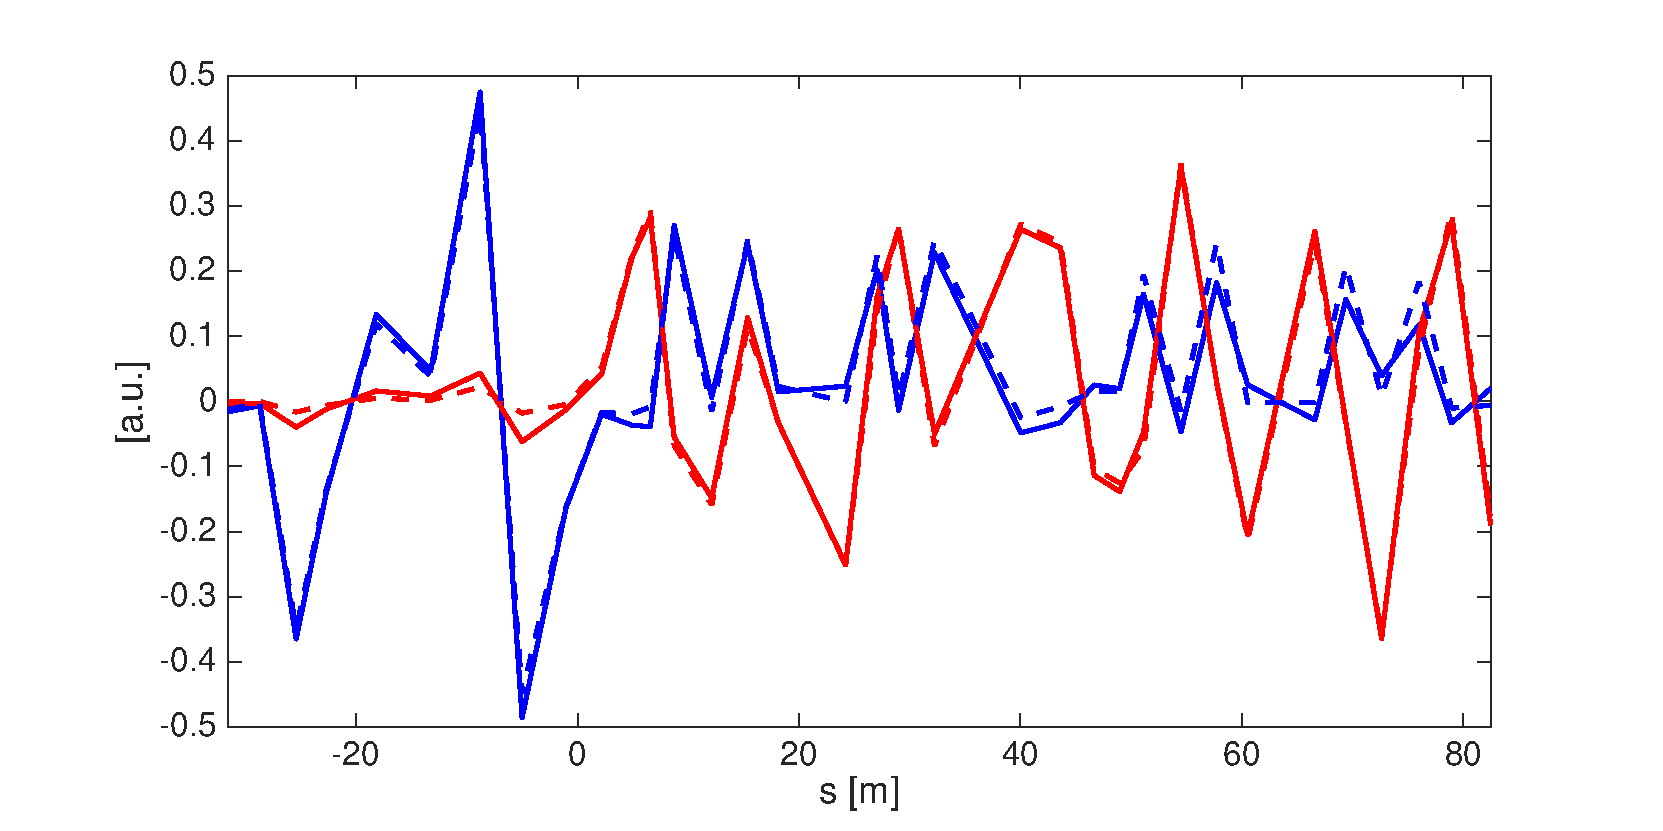
\includegraphics[width=0.66\textwidth]{obtainedSingularDirectionsV3.eps}
\label{fig:septaJitterAnalysisResponses}
}
\\%\qquad
\subfloat[]{
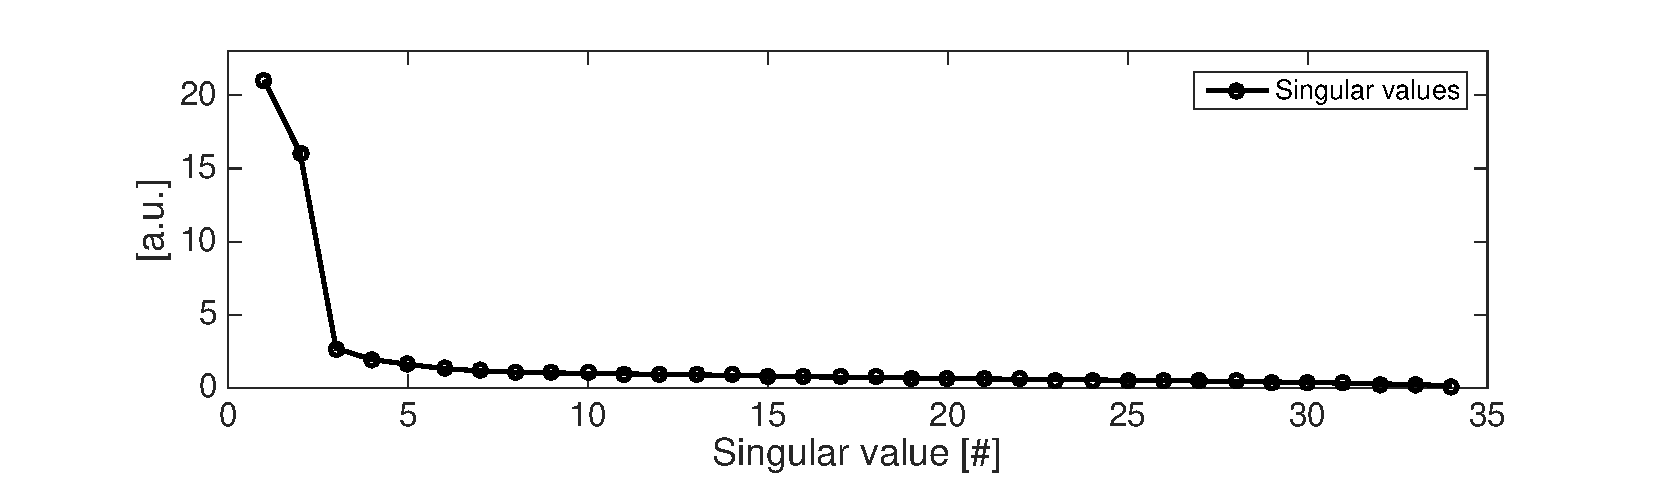
\includegraphics[width=0.66\textwidth]{genericSVDspectrum.eps}
\label{fig:septaJitterAnalysisSpectrum}
}
\caption{Example of jitter identification near the CR injection septa at CTF3.
%\protect\subref{fig:septaJitterAnalysisResponses} on the horizontal axis are the
different BPMs in that area.
\protect\subref{fig:septaJitterAnalysisResponses} on the horizontal axis is the position
of the available BPMs in the area with respect to the septa position ($s = 0$~m).
On the vertical axis is the normalised transverse orbit response under the effects of
septa variation (dashed-red line) and beam-energy variation (dashed-blue line).
The blue and red solid lines are the first and second singular directions of the SVD/PCA
analysis conducted on 100 consecutive beam orbits. 
\protect\subref{fig:septaJitterAnalysisSpectrum} the singular values spectrum of the
associated SVD decomposition.}
\label{fig:septaJitterAnalysis}
\end{figure}
%

It is clear that PCA can be a powerful method to measure and cross-check the dispersion
pattern,
as well as to identify other possible sources of orbit jitter.
This method has been implemented and successfully used in the dispersion monitor tool
developed at CTF3.


\subsubsection{Non-linear dispersion measurement}
%
In general one assumes that the beam orbit is linearly dependent on energy variations,
and practically this is most of the time a fair assumption.
Actually one should expect an inversely proportional dependence on the energy of the beam
(to some power), which is due to the kicks given to the beam from the magnetic elements
of the lattice (see~\cite{bib:DavideThesis}).
This means that for high energy variation and strong optics (like in CTF3) one might
expect non-linearities.
%
One might then wonder how the natural energy spread of the beam could interfere with the
measurement of the beam position,
and so with the dispersion measurement as a difference between two beam positions
readings.
If one assumes that the beam has a Gaussian energy distribution, then when the beam is
crossing a location affected by a generic non-linear dispersion the average beam position
is defined as:
%
\begin{align}
\langle x \rangle &=
\int_{-\infty}^\infty \mathrm{d}\frac{\Delta p}{p_0} \left[
D_x \frac{\Delta p}{p_0} +
DD_x \left(\frac{\Delta p}{p_0}\right)^2 +
DDD_x \left(\frac{\Delta p}{p_0}\right)^3 +
\cdots \right] \times \nonumber \\
&\qquad  \frac{1}{\sqrt{2\pi} \sigma_{\Delta p/p_0} } \exp \left( -\frac{1}{2} \left(\frac{\Delta p/p_0 - \langle \Delta p/p_0 \rangle}{\sigma_{\Delta p / p_0}} \right)^2 \right)
\label{eq:meanPosInNonLinDispStart}
\end{align}
%
where $D_x$, $DD_x$, ... are the linear and non-linear coefficients of the dispersion.
All integrals in Eq.~\ref{eq:meanPosInNonLinDispStart} are the non-central moments of the
Gaussian distribution.
This leads to:
%
\begin{align}
\langle x \rangle &=
D_x \langle \frac{\Delta p}{p_0} \rangle +
DD_x \left( \langle \frac{\Delta p}{p_0} \rangle^2 +  \sigma_{\Delta p / p_0}^2 \right) +
DDD_x \left( \langle \frac{\Delta p}{p_0} \rangle^3 +  3 \langle \frac{\Delta p}{p_0} \rangle \sigma_{\Delta p / p_0}^2
\right) +
\cdots
\label{eq:meanPosInNonLinDisp}
\end{align}
%
Equation~\ref{eq:meanPosInNonLinDisp} clearly shows that indeed the average beam position
is affected by the
beam-energy spread in the case of non-linear dispersion.
For the dispersion measurement one actually needs the orbit difference between two beams
with different energies, which
turns out to be:
%
\begin{align}
\Delta \langle x \rangle &=
D_x \Delta \langle \frac{\Delta p}{p_0} \rangle +
\left( DD_x + 3 DDD_x \sigma_{\Delta p / p_0}^2 \right) \Delta \left( \langle \frac{\Delta p}{p_0} \rangle^2 \right) +
\nonumber \\
&\qquad + \left( DDD_x + \cdots \right) \Delta \left( \langle \frac{\Delta p}{p_0} \rangle^3 \right) + \cdots
\label{eq:deltaPosInMultiOrderDispersion}
\end{align}
%
Similarly to the procedures described in Section~\ref{sub:detailDispMeas} one can then
collect a series of orbit differences under the effect of measurable energy variations,
and fit the \emph{linear} coefficients of 
Eq.~\ref{eq:deltaPosInMultiOrderDispersion} with respect to the \emph{powers} of the
energy variations and extract the linear dispersion coefficient $D_x$, which is $not$
affected by higher order dispersion and/or by the \emph{Gaussian} energy spread
$\sigma_{\Delta p / p_0}$.
Equation~\ref{eq:deltaPosInMultiOrderDispersion} highlights also other observations.
If for example the third order dispersion $DDD_x$ is negligible, then also the second
order dispersion is accessible with reasonable precision.
However the higher order the non-linear term, the more the energy spread of the beam might
affect the measurement.

At CTF3 the non-linear behaviour of the dispersion can be visible in areas with high
dynamic aperture, for example at the end of the linac after the Stretching Chicane.
Figure~\ref{fig:nonLinearitiesAfterFrascati}\subref{fig:nonLinearitiesAfterFrascatiMAD}
shows the expect non-linear dispersion at three BPMs after the Frascati chicane, which is
normally set with a strong optics ($R_{56} = 0$ optics).
The simulation is performed by considering a random displacement of the quadrupoles in the
line of the order of $100 \mu m$, which is the typical alignment precision of CTF3. 
Figure~\ref{fig:nonLinearitiesAfterFrascati}
\subref{fig:nonLinearitiesAfterFrascatiMeasure} shows a real measurement performed in
2014: the beam energy variation on the $x$ axis is computed from the horizontal beam
position at the first dispersive BPM in the Frascati chicane.
%
\begin{figure}[h]
\centering
\subfloat[]
 {
  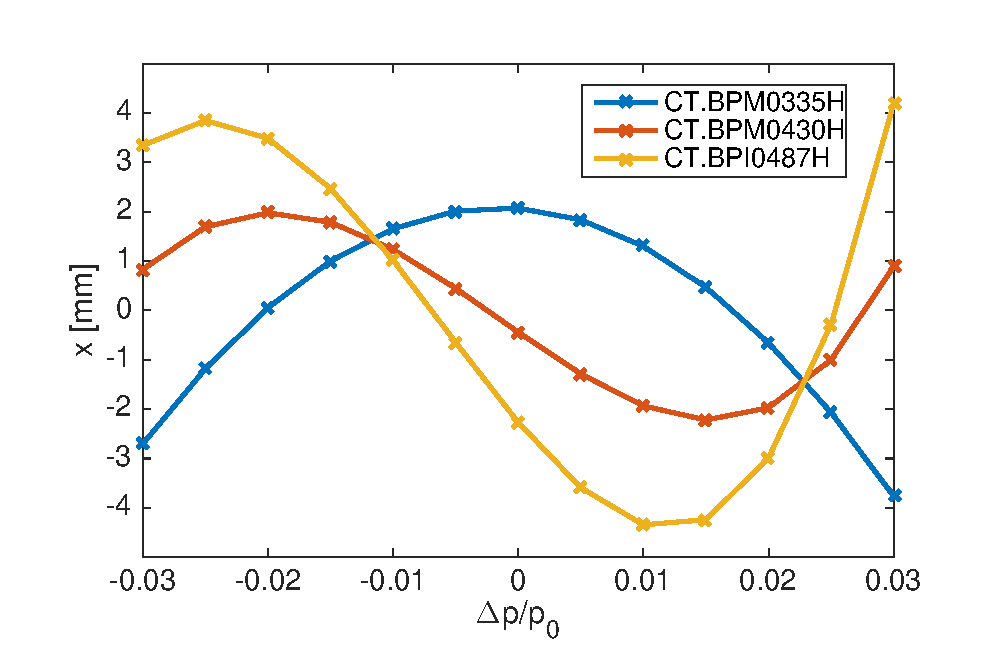
\includegraphics[width=0.45\textwidth]{simulations.eps}
  \label{fig:nonLinearitiesAfterFrascatiMAD}
 }
\qquad
\subfloat[]
 {
   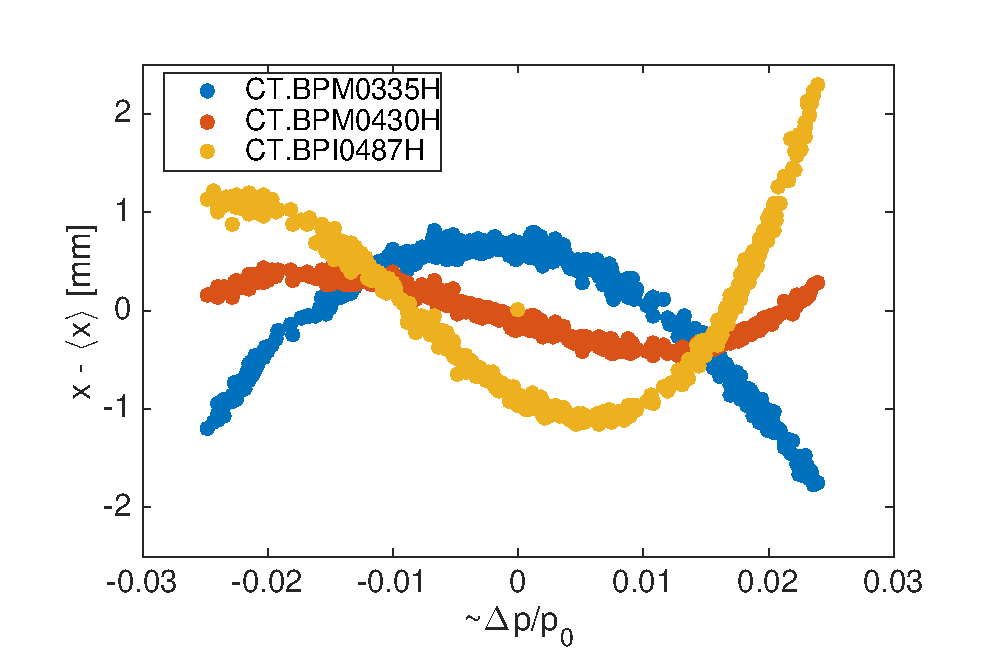
\includegraphics[width=0.45\textwidth]{measurements.eps}
   \label{fig:nonLinearitiesAfterFrascatiMeasure}
 }
\caption{Example of non-linear dispersion measurement at the end of the linac at CTF3.
         \protect\subref{fig:nonLinearitiesAfterFrascatiMAD} the MAD-X simulation of the single
         particle horizontal position as a function of the momentum error at three different BPMs
         installed in the area,
         and whose name is specified in the legend.
         \protect\subref{fig:nonLinearitiesAfterFrascatiMeasure} a measurement of the average beam
         momentum as a function of the beam-momentum error.
         The measurement has been performed at the same BPMs simulated in
         \protect\subref{fig:nonLinearitiesAfterFrascatiMAD}.
         For each BPM the total mean position has been subtracted.
}
\label{fig:nonLinearitiesAfterFrascati}
\end{figure}
%
Even though the two plots in Figure~\ref{fig:nonLinearitiesAfterFrascati} have different vertical axis scales,
the non-linear behaviour of the orbit dependence on the beam energy is extremely similar between measurement and simulation.
The factor 2 scaling difference between the two plots is not justified by the effect presented in Eq.~\ref{eq:deltaPosInMultiOrderDispersion},
but it could be attributed to calibration error of the BPMs, which was suspected but never verified. 
Still one can state that at CTF3 non-linear energy effects are present and at least qualitatively measurable.


\subsubsection{Application features}
%
The \emph{onlineDispersion} MATLAB application developed at CTF3 implements all the
measurements described in the previous sections. % \ref{sub:detailDispMeas}. 
The common ingredient for all these measurement is to collect a certain number of
consecutive orbits.
At each new beam shot a new orbit is collected, stored in a circular buffer of the desired
size, and the dispersion calculation is performed on the stored data and the Graphical
User Interface (GUI) is updated.
It turned out that the ``online'' approach adopted is very useful to obtain an immediate
feedback on the quality of the measurement even after only a few shots.
%
A full list of the application features implemented can be summarised as follows:
%
\begin{itemize}
\item
Measurement and history of the estimated energy error ($\Delta p_i/p_0$) as the beam
position at a reference (dispersive) BPM, normalised by the nominal dispersion expected at
that location.
\item
Ability to wiggle the beam current and/or a set of selected magnets with definable
amplitudes and steps.
\item
Fit of the dispersion as the linear (or non-linear) correlation of each BPM's data with
respect to: 
the energy as measured at the reference BPM,
or the beam current as measured at the exit of the Drive Beam injector,
or the scaling of the specified magnets.
\item
PCA analysis of the acquired orbits and the singular value spectrum is always visible on
the application GUI.
\item
Detailed view of a generic SVD analysis (Eq.~\ref{eq:svdDecompositionOfOrbitsGeneric}) of
the acquired orbits, including the display of the weighted singular directions in the
orbit space (columns of matrix $\mathbf{U}$) and time space (columns of matrix
$\mathbf{V}$).
\item
Detailed view, by scatter plot, of the correlation between a selected BPM and either the
reference BPM or the magnet scaling or the beam current scaling.
\item
Measurement and history of the ``dispersive'' component of the mean beam orbit.
This is computed simply by operating the scalar product between the measured dispersion
and the mean orbit as measured by the BPMs.
A dispersive component different from zero might be a sign that the optics is not matched
to the mean energy of the beam.
\end{itemize}
%
The main graphical interface of the application is illustrated in
Figure~\ref{fig:onlineDispersionGUI}.
The final implementation consists of a MATLAB compiled executable that loads a
user-editable XML\footnote{eXtensible Markup Language.} configuration file.
In this way the same application can be used to measure the dispersion in any desired
beamline of CTF3.
The XML configuration file contains mainly the list of BPMs to monitor and the list of
magnets to use for the magnet-scaling measurement type.
All the details of the implementation and possible options and setup of the application
are beyond the scope of the present work.
It is worth mentioning that a separate GUI, not shown here, can display the detailed SVD
analysis of the acquired orbits.
This last GUI turned out to be extremely useful when more than one outstanding singular
value is detected: 
by looking at the detected singular direction in the observable space one has some hints
on the source of additional orbit jitter that is not correlated to the beam energy
variation. 

%%%%%%%%%%%%%%%%%
%
\begin{sidewaysfigure}
\centering
\begin{tikzpicture}
    \node[anchor=south west,inner sep=0] (image) at (0,0) 
    {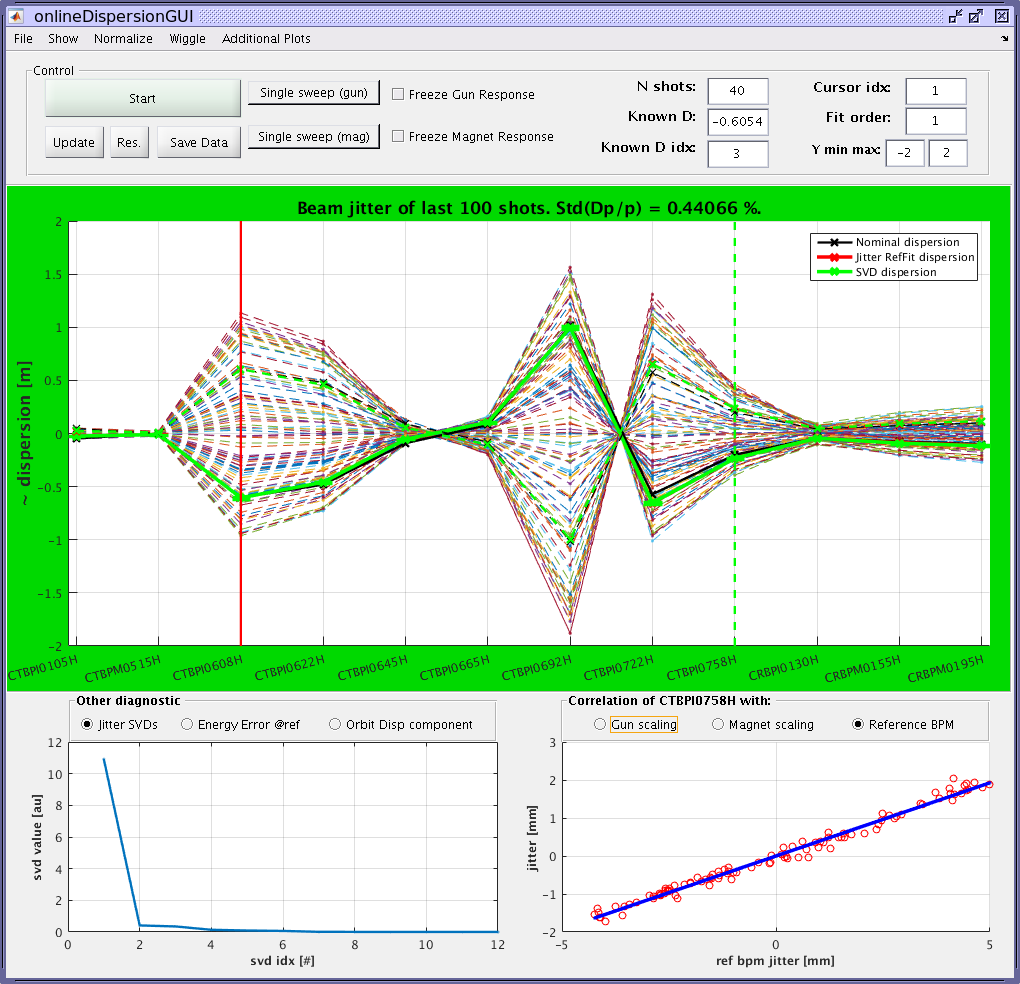
\includegraphics[width=0.55\textwidth]{newDispInterface.png}};
    \begin{scope}[x={(image.south east)},y={(image.north west)}]
    %
        % main traces
        \draw[orange,ultra thick,rounded corners, fill=red!20, fill opacity=0.3]
         (0.01,0.302) rectangle (0.99, 0.77);
        \draw[orange,ultra thick,->] (0.99,0.55) -- (1.03,0.55) node [right, black,
         align=left, text width=5cm] 
        {Main view with all the acquired jitter traces and dispersion fits. On the $x$
        axis are the BPM names, on the $y$ axis the approximate dispersion. \\ 
        The jitter traces are in arbitrary units and scaled to fit the measured dispersion
        amplitude.};
        % bottom right
        \draw[orange,ultra thick,rounded corners, fill=red!20, fill opacity=0.3]
        (0.505,0.01) rectangle (0.99, 0.298);
        \draw[orange,ultra thick,->] (0.99,0.15) -- (1.03,0.15) node [right, black,
        align=left, text width=5cm] 
        {Jitter at the selected BPM and linear fit versus the chosen parameter: either
        beam current variation, or magnet scaling, or \emph{jitter at reference BPM}.};
        % bottom left
        \draw[orange,ultra thick,rounded corners, fill=red!20, fill opacity=0.3]
        (0.01,0.01) rectangle (0.495, 0.298);
        \draw[orange,ultra thick,->] (0.01,0.15) -- (-0.03,0.15) node [left, black,
        align=right, text width=5cm] 
        {Advance analysis: either \emph{singular values spectrum}, or history of the mean
        energy variations at reference BPM, or history of nominal dispersion component of
        the mean orbit.};
        %\draw[green!70!red, thick,->] (0.8,0.4) -- (0.7,0.3); % to indicate selected bpm
        % title of middle plot
        \draw[orange,ultra thick,rounded corners, fill=red!20, fill opacity=0.3]
        (0.25,0.77) rectangle (0.76, 0.81);
        \draw[orange,ultra thick,->] (0.25,0.795) -- (-0.03,0.6) node [left, black,
        align=right, text width=5cm] 
        {Number of shots collected and standard deviation of the observed energy
        jitter assuming nominal dispersion at the reference BPM.};
        \draw[orange,ultra thick,rounded corners, fill=red!20, fill opacity=0.3]
        (0.01,0.82) rectangle (0.55, 0.97);
        \draw[orange,ultra thick,->] (0.01,0.88) -- (-0.03,0.88) node [left, black,
        align=right, text width=5cm] 
        {Main control for the application and access to advanced menu for fine tuning of
        parameters and detailed analysis.};
        % top right controls
        \draw[orange,ultra thick,rounded corners, fill=red!20, fill opacity=0.3]
        (0.57,0.82) rectangle (0.99, 0.93);
        \draw[orange,ultra thick,->] (0.99,0.88) -- (1.03,0.88) node [right, black,
        align=left, text width=5cm] 
        {Specification of buffer size and main assumption on dispersion at the selected
        reference BPM.};
    %
    \end{scope}
\end{tikzpicture}
\caption{Online dispersion monitor. Main graphical interface.}
\label{fig:onlineDispersionGUI}
\end{sidewaysfigure}
%
%%%%%%%%%%%%%%%%%







% > \tb{Taken from Davide's LINAC16 paper}
% > 
% > The dispersion in a transfer line can be measured by 
% > changing the momentum of the beam with respect to 
% > the nominal momentum ($p_0$) the line is tuned for, 
% > and then measuring the mean orbit deviation.
% > %
% > The observed orbit displacement ($\Delta x$) can be expressed as:
% > %
% > \begin{align}
% > \Delta x = D_x \frac{\Delta p}{p_0} +
% >  DD_x  \left(\frac{\Delta p}{p_0}\right)^2 + 
% >  o\left(\left(\frac{\Delta p}{p_0}\right)^3\right).
% > \label{eq:simpleDispersionDefinition}
% > \end{align}
% > %
% > One can then fit the coefficients $D_x$, which is the linear dispersion, 
% > and if necessary also the higher order terms (e.g. $DD_x$).
% > Practically the measurement of $D_x$ is often sufficient to 
% > spot errors or mismatches in a beam line.
% > 
% > %
% > In transfer lines where dispersion is expected by design another 
% > interesting observable is what we call the ``nominal'' linear dispersion,
% > i.e. the orbit response while scaling \emph{only} the bending magnets. 
% > This quantity is not affected by quadrupole misalignments and orbit errors,
% > hence it is a direct measurement, with opposite sign, 
% > of $D_x$ in Eq.~\ref{eq:simpleDispersionDefinition} for the ideally aligned 
% > linear machine \cite{bib:DavideThesis}.
% > Note that the measured quantity is \emph{not} the actual dispersion 
% > experienced by the beam,
% > but it is the dispersion contribution of the bending magnets which, 
% > in an ideal-linear machine, are the only sources of dispersion.
% > This observable turns out to be useful for optics verification and 
% > it can be used to define the target dispersion for DTS.
% > 
% > %
% > At CTF3 a MATLAB application to perform online measurements of 
% > linear and non-linear dispersion has been developed \cite{bib:DavideThesis}.
% > The relative energy of the beam with respect to the beam lines can be 
% > varied mainly in three ways:
% > %
% > \begin{itemize}
% > \item
% > By scaling all the magnetic elements in the line. Note that this method 
% > would not reveal the \emph{incoming} dispersion, 
% > but only the dispersion generated within the section of beam line being scaled.
% > \item
% > By scaling the beam current delivered by the thermionic gun. 
% > Since the Drive Beam linac relies on fully loaded accelerating structures, 
% > one can assume a linear correlation between beam current and 
% > beam acceleration \cite{bib:CTF3DesignReport}.
% > \item
% > By varying the phase and/or power of the accelerating structures in the linac, 
% > which has a similar effect as scaling the beam current.
% > \end{itemize}
% > %
% > The more convenient method is to vary the beam current. 
% > 
